\chapter{Risultati}
\section{Convergenza}


\section{Foto}

\begin{figure}[!htbp]
        \centering%
        \subfigure[m=9.]%
          {\label{fig: slice9}\includegraphics[scale=0.15]{DDDD_ADR/HiMod9slice.eps}}\qquad
        \subfigure[m=16.]%
          {\label{fig:slice16}\includegraphics[scale=0.15]{DDDD_ADR/HiMod16slice.eps}}\qquad
		\subfigure[m=25.]%
          {\label{fig:slice25}\includegraphics[scale=0.15]{DDDD_ADR/HiMod25slice.eps}}\qquad
          \subfigure[FEM.]%
          {\label{fig:sliceFEM}\includegraphics[scale=0.15]{DDDD_ADR/FEMslice.eps}}\qquad
        \caption{Caso test DDDD\_ADR sezione XZ}
        \label{fig:DDDD_ADR slice}
\end{figure}

\begin{figure}[!htbp]
        \centering%
        \subfigure[Solusione FEM.]%
          {\label{fig: FEMsol}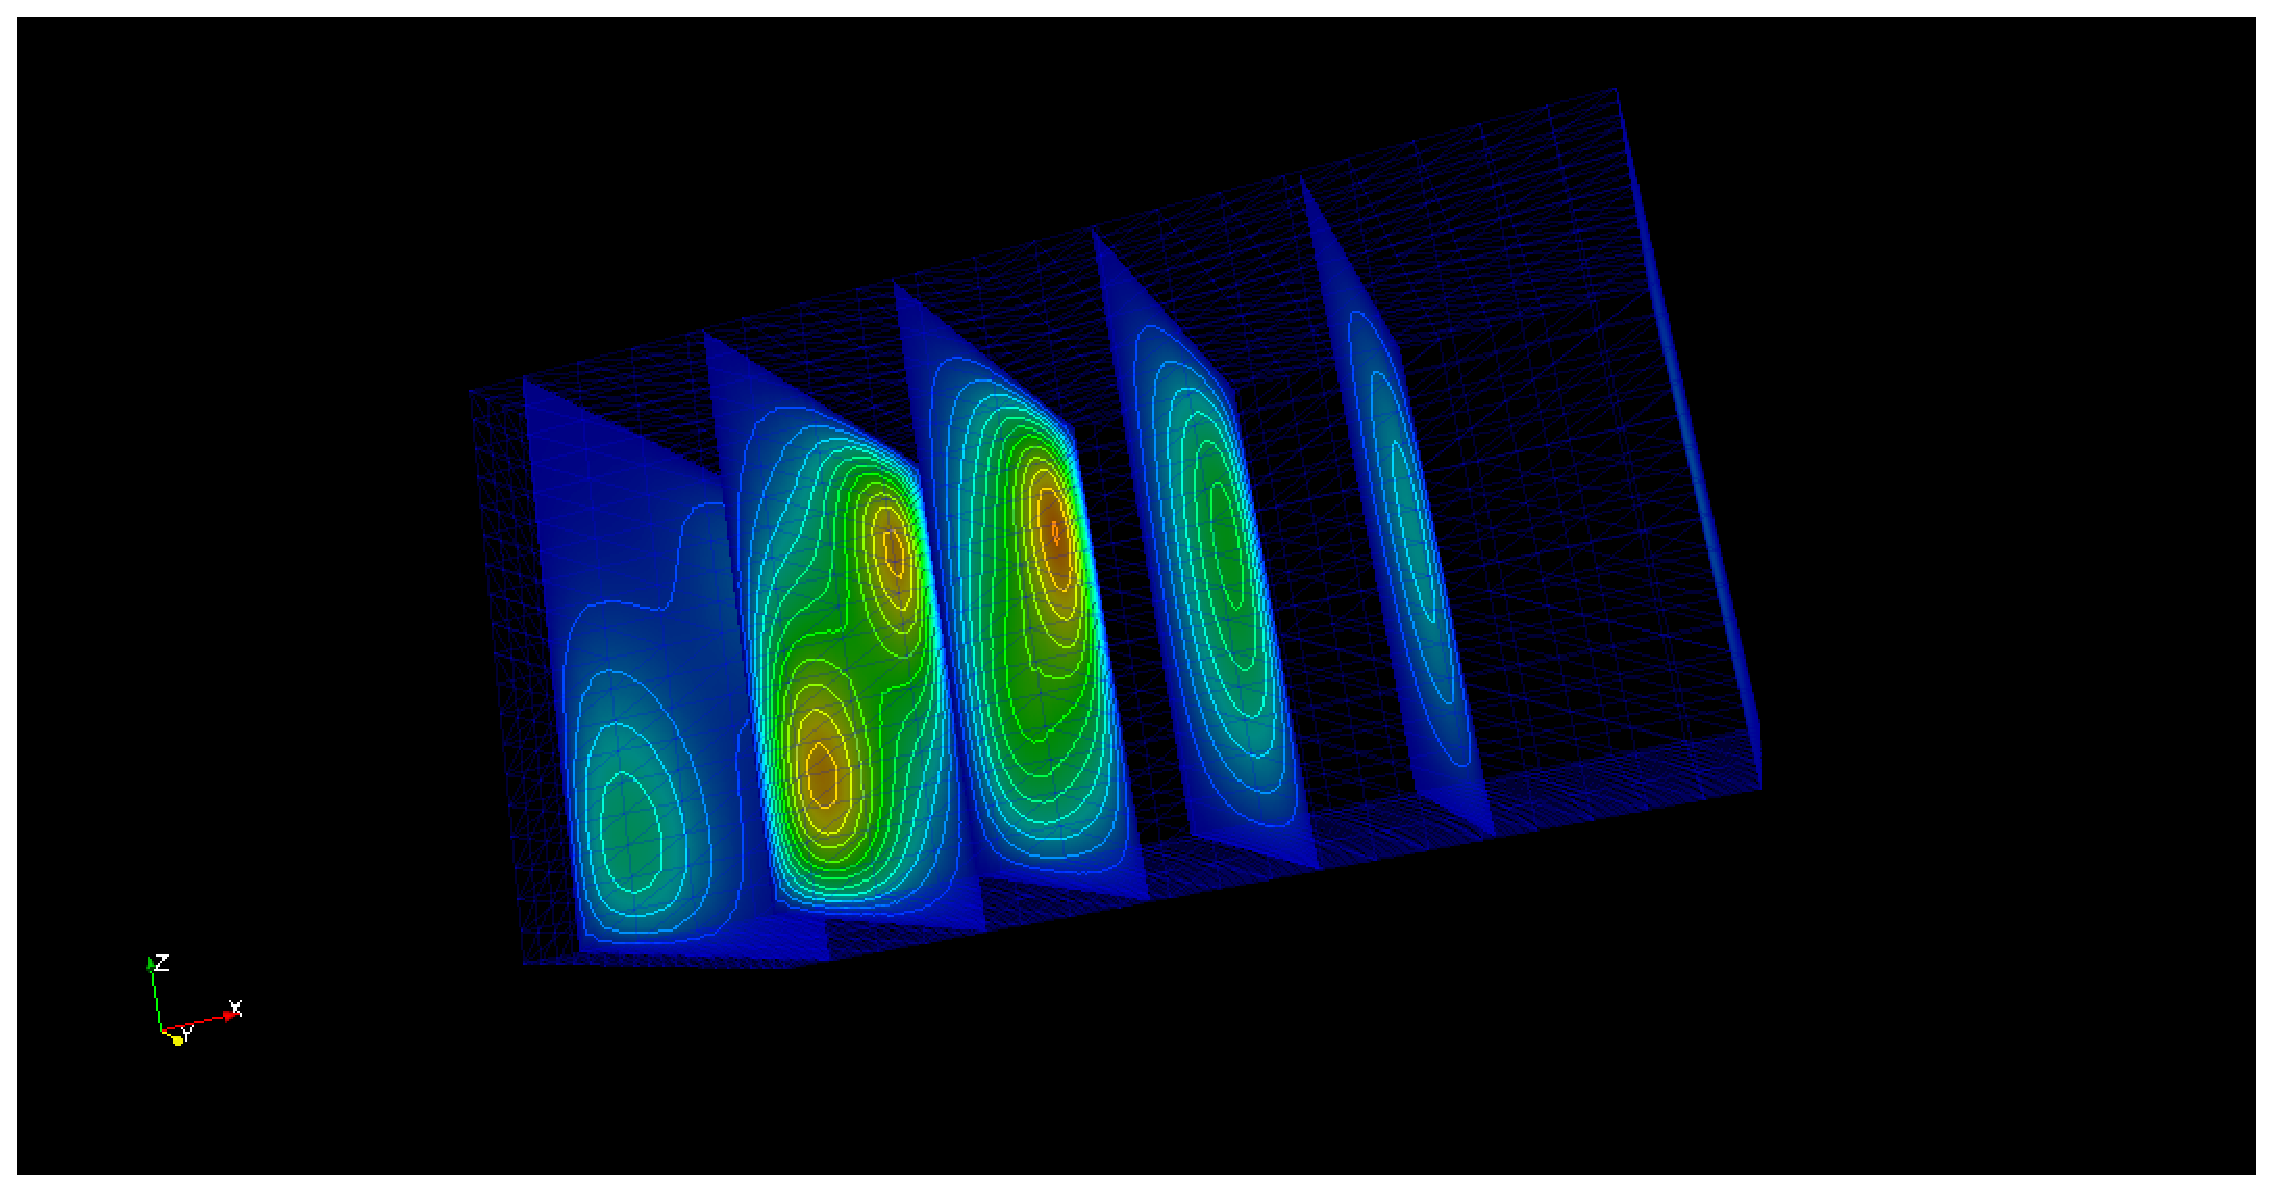
\includegraphics[scale=0.36]{DDDD_ADR/FEM.eps}}\qquad
        \subfigure[Solusione HiMod m=50.]%
          {\label{fig:HiMod50sol}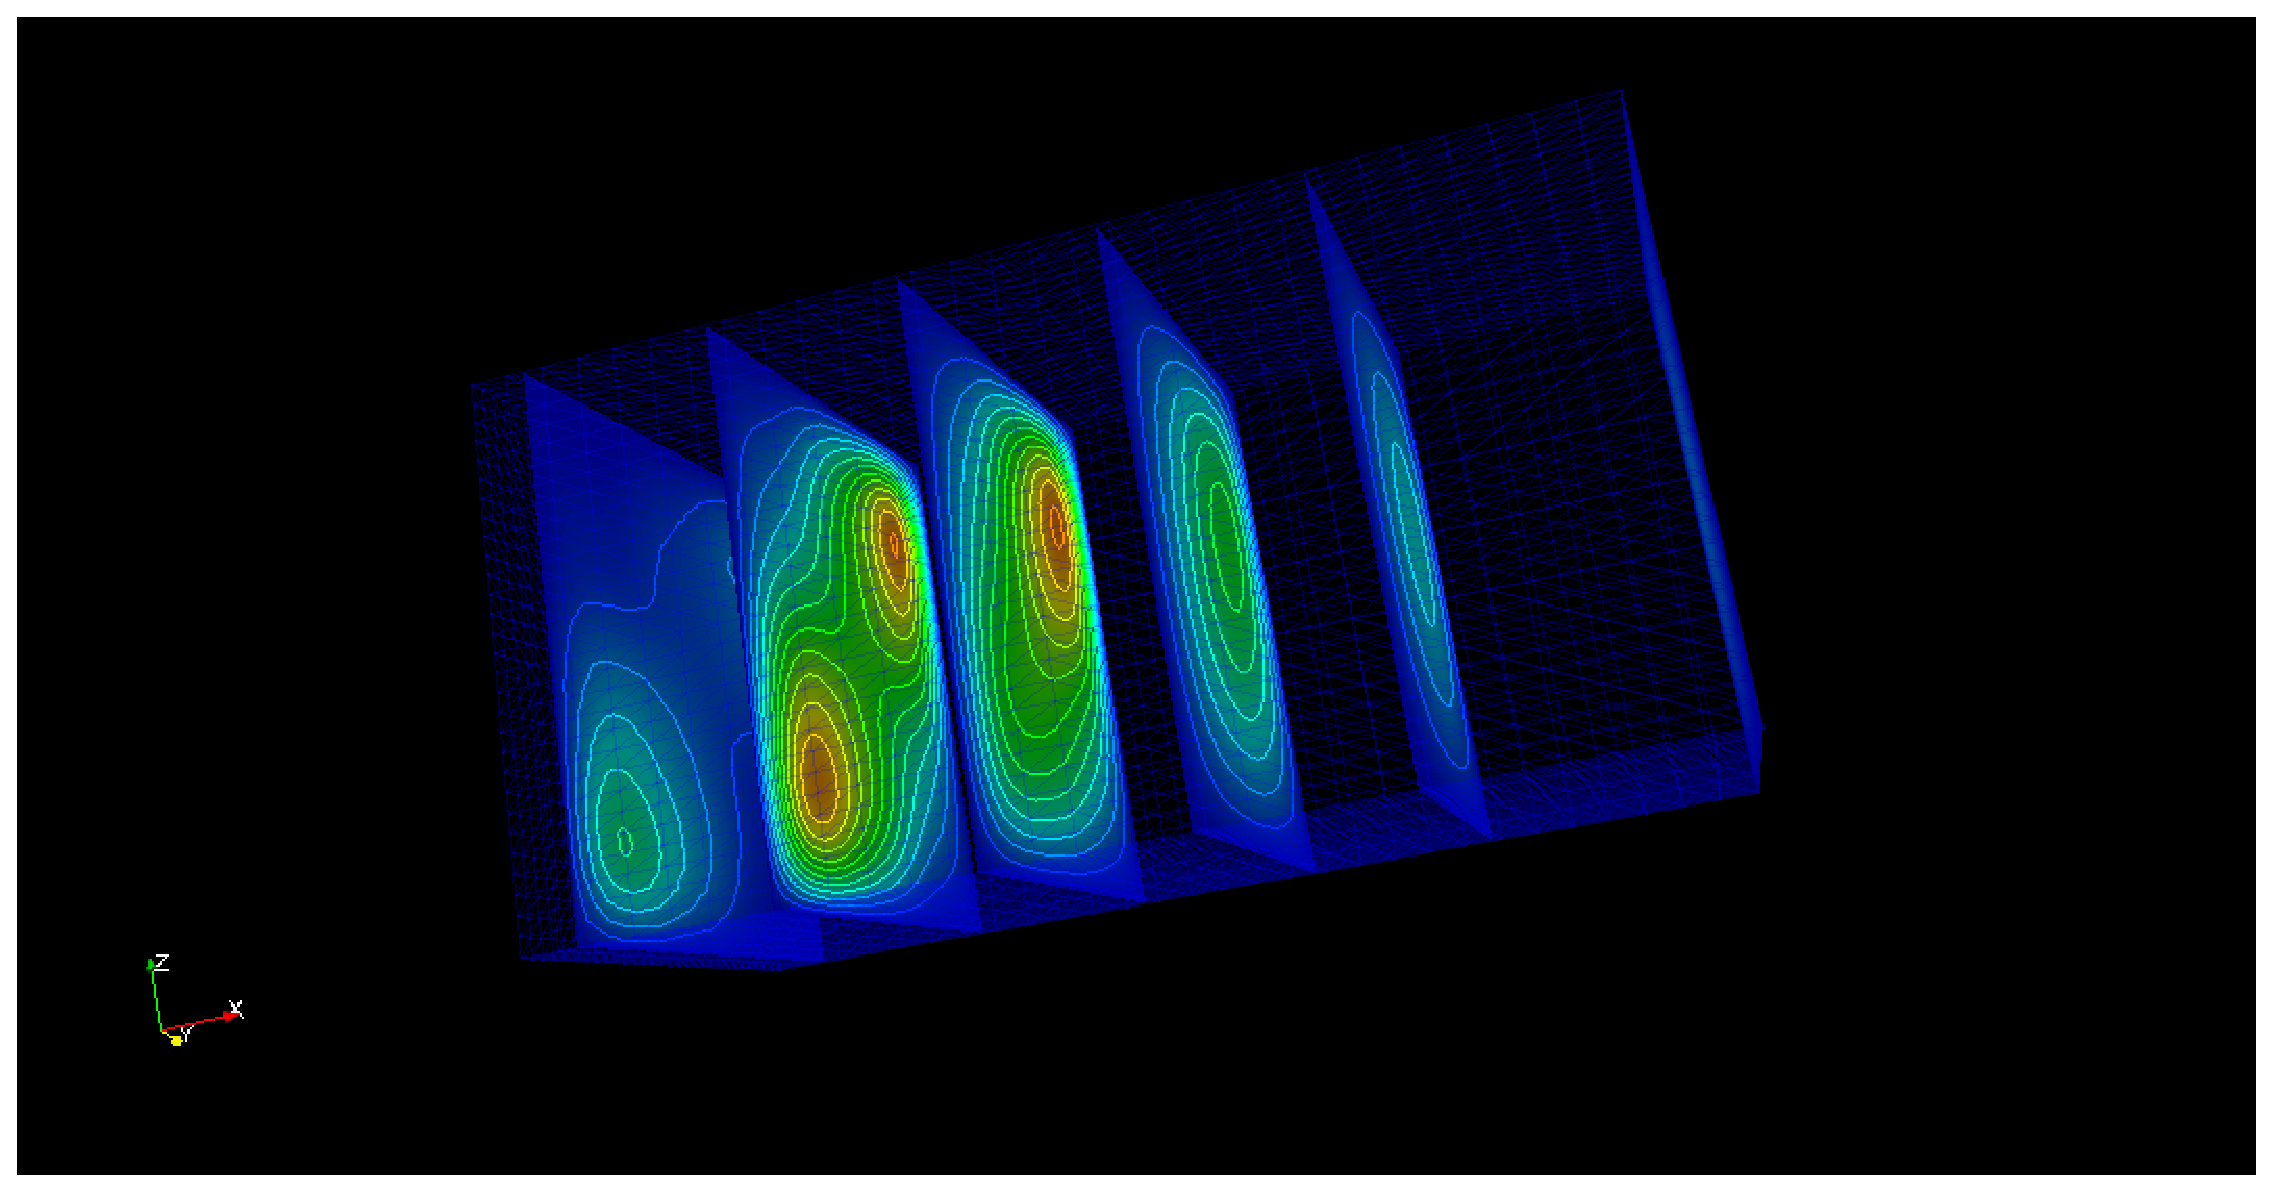
\includegraphics[scale=0.36]{DDDD_ADR/HiMod50.eps}}\qquad
        \caption{Caso test DDDD\_ADR}
        \label{fig:DDDD_ADR}
\end{figure}